% POT.tex      pdflatex ZhCvGo15
% Diffuse globally, compute locally: a cyclist tale
% Tingnan Zhang, Daniel I. Goldman and Predrag Cvitanovi\'c

% \subsection{Periodic orbit theory}
% \label{s-POT}

\Po\ theory of deterministic diffusion, introduced in
\refrefs{art91,LorentzDiff}, exploits the fact that the periodic Lorentz
gas can be constructed by putting together translated copies of an
elementary cell. Therefore quantities characterizing global dynamics,
such as the Lyapunov exponents and the diffusion tensor, can be computed
from the dynamics restricted to the elementary cell, as shown numerically
in \refref{CGS92}.

However, when this elementary cell is itself invariant under a discrete
symmetry group $G$ the lattice can be tiled into images under $G$ and the
lattice translations of a fundamental domain.

In \refrefs{art91,LorentzDiff,CGS92,Artuso94,CBdiffusion} it was shown that
deterministic diffusion tensor in the {\em periodic} Lorentz gas can be
expressed in terms of (relative) \po s, and exact \cycForm\ for such
global dynamical averages as Lyapunov exponent and diffusion tensor were
derived, using only the dynamics in the elementary cell. For any
dynamical system that has translational symmetry,the full state space
$\hM$ (i.e., both spatial coordinates and momenta) has aperiodic tiling
\[ %beq
\hM=\bigcup_{ \hn \in T} \pS_{\hn},
\] %eeq
by {\em translating} $\pS_{\hn}$ of an {\em elementary cell} $\pS$, with
$T$ the abelian group of lattice translations.

In the context of Lorentz gas system, the elementary cell is the
hexagonal region centered at the scatterer, see
\reffig{fig-chaoticBouncing} (a). The dynamics restricted inside the
elementary cell is understood as the periodic boundary condition: when
the particle leaves the edge of the hexagon cell, it immediately enters
the region again from the opposite edge. We distinguish two types of
diffusive behavior; the {\em infinite horizon} case, which allows for
infinite length flights, and the {\em finite horizon} case, where any
free particle trajectory must hit a disk in finite time. The transition
between horizon and infinite horizon is controlled by the ratio of $w/r$,
where $w$ is the gap between nearest pair of disk and $r$ the radius of
the disk.

We now relate the dynamics in $\pS$ to diffusive properties of the
Lorentz gas in $\hM$. Let $\hx(t)\,=\,\hflow{t}{\hx_0}$ denotes the point
in the global space $\hM$ reached by the flow in time $t$.
$x(t)\,=\,\flow{t}{\xInit}$ denotes the corresponding flow in the
elementary cell; the two are related by
\beq
\hn_t(\xInit)=\hflow{t}{\xInit} - \flow{t}{\xInit} \in T \,,
\ee{l-diff-hatn1}
the translation of the endpoint of the global path into the elementary cell $\pS$.

Fix a vector $\beta \in \reals^d$, where $d$ is the dimension of
the{\statesp}. We will compute the diffusive properties of the Lorentz
gas from the leading eigenvalue of the Rulle-Frobenius-Perron \evOper\
\beq
\eigenvL(\beta)\,=\, \lim_{t \rightarrow \infty} \frac{1}{t} \log \langle
e^{\beta \cdot (\hx(t) -x) } \rangle_\pS ~, \quad
\label{eq-diff-1}
\eeq
where the average is over all initial points in the elementary cell, $x
\in\pS$. If all odd derivatives vanish by symmetry, there is no drift and
the second derivatives
\begin{widetext}
\beq
2d D_{ij} = \left . {\frac{\partial}{\partial \beta_i}} {\frac{\partial}
{\partial \beta_j}} \eigenvL(\beta)\right\vert_{\beta=0} \,=\,\lim_{t\rightarrow
\infty} {\frac{1}{t}} \langle {(\hx(t) -x)_i (\hx(t) -x)_j } \rangle_\pS ~,
\eeq
\end{widetext}
yield a diffusion matrix.  This symmetric matrix can, in general, be
anisotropic(\ie, have $d$ distinct eigenvalues and eigen\-vectors). The
spatial diffusion constant is then given by the Einstein relation
\beq
D\,=\,{1\over 2 d} \sum_i \left .{{\partial}^2 \over {\partial
      \beta^2_i}} \eigenvL(\beta)\right |_{\beta=0} \,=\,
\lim_{t\rightarrow \infty} {1\over{2d t}} \langle {(\hat{q}(t) -q)^2 }
\rangle_\pS~ ~,
\eeq
where the $i$ sum is restricted to the spatial components $q_i$ of
the{\statesp} vectors $x=(q,p)$, \ie, if the dynamics is Hamiltonian, the
sum is over the $d$ degrees of freedom.
\PC{2014-11-18}{reinstate mass, velocity, size to get $\beta$, $m$, $\sigma$
    dependencies right?}

We now turn to the connection between diffusion and periodic orbits in
the elementary cell. It was shown in \refref{CGS92} that the ensemble
average in\refeq{eq-diff-1} can be written as an integral over the
elementary cell
\beq
\langle e^{\beta\cdot(\hx(t)-x)} \rangle
   = \frac{1}{\vert \pS \vert}\int_{x,y\in \pS} dxdy {\cal L}^t(y,x),
\eeq
given the linear \evOper operator
\beq
{\cal L}^t(y,x) = e^{\beta\cdot(\hx(t)-x)}\delta(y-x(t))
\label{eq-eOper}
\eeq
The interesting dynamical averages is determined by the spectrum of the operator
\beq \det(\eigenvL - \Lop) \,=\,\prod_{p} \exp \left(
  - { \sum_{r=1}^\infty {1 \over r} { e^{(\beta \cdot \hn_p- s
        \period{p}) r} \over \oneMinJ{r} }
  } \right) \,,
\ee{lor-diff-14}
or the corresponding \dzeta\
\beq
1/\zeta(\beta, s)\,=\,\prod_{p}\left( 1 - \frac{e^{(\beta \cdot \hn_p-
      s \period{p})}}{|\ExpaEig_p|} \right) ~,
\label{zeta-diff}
\eeq
where $\period{p}$ is the period of the cycle and $\ExpaEig_p$ the
product of expanding eigenvalues of the cycle\rf{DasBuch}.

The \dzeta\ \cycForm\ for the diffusion constant, zero mean drift
$ \expct{ \hat{x}_i } = 0 \,, $ is given by
 \beq D \,=\,{1 \over 2 d}
{ \expct{\hat{x}^2}_\zeta \over \expct{\period{}}_\zeta } \,=\,{1
  \over 2 d } \, {1 \over \expct{\period{}}_\zeta} \sumprime
\frac{(-1)^{k+1} (\hn_{p_1}+ \cdots+ \hn_{p_k})^2}
{|\ExpaEig_{p_1}\cdots \ExpaEig_{p_k}|} \, ,
\label{eq-ecDiffCoef}
\eeq
where the sum is over all distinct non-repeating combination of prime
cycles (in the elementary cell). The derivation is standard, still the
formula is strange.Diffusion is unbounded motion across an infinite
lattice; nevertheless, the reduction to the elementary cell enables us to
compute relevant quantities in the usual way, in terms of periodic
orbits.

\subsection{Cycles in the elementary cell}
\begin{figure}
  \begin{center}
    (a)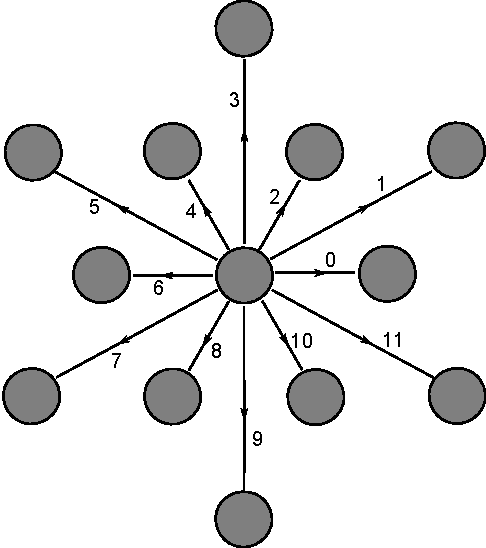
\includegraphics[width=0.27\textwidth]{diffuseDiskDirectionsElCell}
    (b)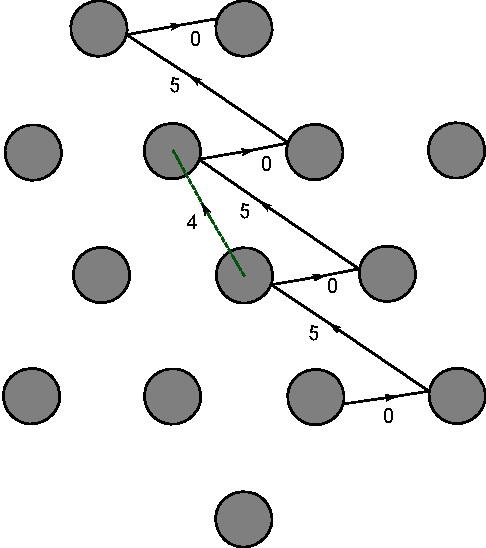
\includegraphics[width=0.27\textwidth]{diffuseDiskDirecsElCell05}
    (c)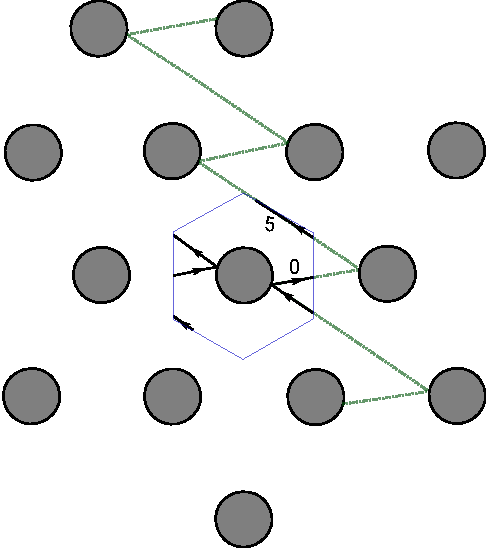
\includegraphics[width=0.27\textwidth]{diffuseDiskDirecsElCell05red}
  \end{center}
  \caption{\label{fig-diskDirectionsElCell}
  Elementary cell symbolic dynamics is obtained by labeling the
  translation vectors connecting the center of the current disk to the
  center of  the next disk. (a) The finite horizon is here imposed by
  limiting jumps from  the center cell to only the short jumps (six even
  labels $0, 2,\cdots,10$) and  the `long jumps' (six odd labels $1,
  3,\cdots,11$). (b) Running mode  \cycle{05} advances by $\hn_4$ per
  period. (c) In the elementary cell this is  a \po\ \cycle{05} of
  topological length 2.
  }
\end{figure}

We use the symbolic dynamics developed in \refref{CGS92} and briefly
review the concepts here. With imposed finite horizon there are 12
possible ways of jump from a disk
(\reffig{fig-diskDirectionsElCell}\,(a)). Any trajectory in the full
space can always be constructed from a series of flights, each belongs to
the 12 ``signature jumps''. In particular, a periodic orbit in the
elementary cell is represented as a repeatable string of such symbols.
For example, the bouncing mode between nearest disks is written as
\cycle{06}, meaning that the periodic orbit is consisted of two
successive flights, one traveling towards right (symbol $0$) and the next
reflecting backwards (symbol $6$).

Periodic orbits in the elementary cell can either be stationary in the
full space that goes back to its original place after completing a full
cycle (e.g., \cycle{06} that represents the bouncing of the particle
between two nearest disk); or can be in a running mode that generates a
net displacement along the trajectory (e.g., \cycle{05},
\reffig{fig-diskDirectionsElCell}\,b and c). The stationary cycles
``trap'' the  particle locally for a finite amount of time while the
running cycles advance it. The final diffusion \refeq{eq-ecDiffCoef} can
be conceptually understood as the result of competition between the two
type of cycles.

With the symbolic dynamics, we then use the least action principle to
compute the periodic orbits\rf{DasBuch}. In a planetary Hamiltonian
billiard system, the Maupertuis' principle indicates that the traveling
length along a cycle is minimized. We can solve the problem by optimizing
the total free flight distance with the constraint that links have to
connect the specific disks visited along the orbit.

Elementary cycles found using this method and the corresponding cycle
expansion calculation results are listed in \reftab{TCELL1}. Although the
diffusion coefficient computed using elementary cycles up to $n_p = 8$
matches the numerical experiment value $0.25$, the convergence is not
promising.

\begin{table}[htbp]
%\begin{center}
\begin{tabular}{|r|r|r|l|l|}
\hline
${n_p}$ & \# cycles & $\zeta$(0,0) & $\lambda$ & D \\ \hline\hline
1      & 0      &   -    &   -  &   - \\
2      & 24     & -0.31697 & 1.330 & 0.375\\
3      & 64     & -0.54152 & 1.435 & 0.339\\
4      & 168    & -0.09764 & 1.902 & 0.284\\
5      & 516    &  0.02334 & 2.324 & 0.215\\
6      & 1589   & -0.00481 & 1.975 & 0.133\\
7      & 5700   & -0.01241 & 1.885 & 0.184\\
8      & 20729  & -0.01006 & 1.785 & 0.247\\ \hline

\end{tabular}
\caption{\label{TCELL1}
Cycle expansion results computed Schreiber 1992 calculation\rf{CGS92} (and
  this paper) in elementary cell.
}
\end{table}

For a simple example, see the chain of baker's maps chain of coupled
baker maps studied in \refref{Gaspard92}.

Some confidence can be gained at this point by applying the above
formula~\refeq{TS:formula} to a trivial system, a

In this case there are only four fixed points, all with
stability $\Lambda_p=1/2$, two of
which give rise to the translations $\hn_{p}=\pm 1$.
As the system is
uniformly hyperbolic, all curvature terms are identically zero,
and the fixed points substituted into \refeq{TS:formula} yield
immediately the correct result $D=1/4$.
